% File tacl2018.tex
% Aug 3, 2018

% The English content of this file was modified from various *ACL instructions
% by Lillian Lee and Kristina Toutanova
%
% LaTeXery is all adapted from acl2018.sty.

\documentclass[11pt,a4paper]{article}
\usepackage[hyperref]{tacl2018} % use ``nohyperref'' to disable  hyperref
% \usepackage[nohyperref]{tacl2018}
% TODO: change for final version
\usepackage{times,latexsym}
\usepackage{url}
\usepackage[T1]{fontenc}
\usepackage{graphicx}
\usepackage{textcomp}

\taclfinalfalse % For camera-ready, replace "\taclfinalfalse" with
% "\taclfinalcopy"

%%%%
%%%% Material in this block can be removed by TACL authors.
% It consists of things specific to generating TACL instructions
\usepackage{xspace,mfirstuc,tabulary,tabularx}

\newcommand{\ex}[1]{{\sf #1}}
\newcommand{\ea}[1]{\textcolor{blue}{\bf\small [#1 --EA]}}
\newcommand{\yt}[1]{\textcolor{cyan}{\bf\small [#1 --YT]}}
\newcommand{\red}[1]{\textcolor{red}{#1}}
% \newcommand{\yt}[1]{\textcolor{blue}{\bf\small [#1 --srallaba]}}



%
\iftaclfinal
\newcommand{\taclpaper}{camera-ready\xspace}
\newcommand{\taclpapers}{camera-readies\xspace}
\newcommand{\Taclpaper}{Camera-ready\xspace}
\newcommand{\Taclpapers}{Camera-readies\xspace}
\else
\newcommand{\taclpaper}{submission\xspace}
\newcommand{\taclpapers}{{\taclpaper}s\xspace}
\newcommand{\Taclpaper}{Submission\xspace}
\newcommand{\Taclpapers}{{\Taclpaper}s\xspace}
\fi

\newif\iftaclinstructions
\taclinstructionsfalse
\iftaclinstructions
\renewcommand{\confidential}{}
\renewcommand{\anonsubtext}{(No author info supplied here, for consistency with
TACL-submission anonymization requirements)}
\fi
%%%% End TACL-instructions-specific macro block
%%%%

\newcommand{\ignore}[1]{}

\newcommand{\Sref}[1]{\S\ref{#1}}
\newcommand{\fref}[1]{Figure~\ref{#1}}
\newcommand{\Fref}[1]{Figure~\ref{#1}}
\newcommand{\tref}[1]{Table~\ref{#1}}
\newcommand{\Tref}[1]{Table~\ref{#1}}

\newenvironment{itemizesquish}{\begin{list}{\labelitemi}{\setlength{\itemsep}{-0.25em}\setlength{\labelwidth}{0.5em}\setlength
{\leftmargin}{\labelwidth}\addtolength{\leftmargin}{\labelsep}}}{\end{list}}

% tables etc
\newcolumntype{b}{X}
\newcolumntype{s}{>{\hsize=.01\hsize}X}
\newcolumntype{m}{>{\hsize=.05\hsize}X}
\usepackage{booktabs}

% \newcolumntype{R}[2]{%
%     >{\adjustbox{angle=#1,lap=\width-(#2)}\bgroup}%
%     l%
%     <{\egroup}%
% }
% \newcommand*\rot{\multicolumn{1}{R{25}{1em}}}
\newcommand*\rot{\rotatebox{45}}


\title{Understanding Code-Mixing in Controlled Dialogues}


% The command \taclfinalfalse suppresses display of the contents of the
% \author{...} command in the generated pdf.
% Replacing that command with "\taclfinalcopy" reveals the author info in the
% generated pdf.
% See tacl2018.sty for other ways to set author info.
\author{
 Template Author\Thanks{The {\em actual} contributors to this instruction
 document and corresponding template file are given in Section
 \ref{sec:contributors}.} \\
 Template Affiliation/Address Line 1 \\
 Template Affiliation/Address Line 2 \\
 Template Affiliation/Address Line 2 \\
  {\sf template.email@sampledomain.com} \\
}

\date{}

\begin{document}
\maketitle
\begin{abstract}
%With the goal of having conversational AI 
To enable naturalistic conversational agents for multilingual users, dialogue systems need to be extended to converse with bilinguals, potentially using multiple languages in an utterance (i.e. code-mixing). 
Yet little is known about human preferences for code-mixing in the context of a dialogue. 
To fill this gap and to study preferred code-mixing styles, we incorporate linguistically-motivated strategies of code-mixing into a rule-based goal-oriented dialogue system.
We collect a corpus of 587 human--computer text conversations between our dialogue system and fluent Spanish--English bilinguals.
From this new corpus, we analyze the amount of elicited code-mixing, types of code-mixing strategies people use, and whether they entrain to the system's code-mixing. 
Based on these exploratory findings, we give recommendations for future code-mixing dialogue systems.
% \yt{if you can complete the sentence with recommendations for future code-mixing dialogue systems it would be great.}

% design a Spanish--English code-mixing dialogue system 
% With these measures, we present analyses of each strategy's effect on the amount of elicited CM and amount of entrainment with respect to dialogue success.

\end{abstract}

\section{Introduction}

Code-mixing\footnote{We use the term ``code-mixing'' throughout this paper, which is an intra-sentential form of code-switching, meaning it occurs within the boundaries of an utterance.} (CM) refers to the phenomenon where people use multiple languages to communicate \citep{sankoff1981formal}.
An example of this is the utterance in Spanish and English: ``\textit{tengo una} [I have a] friend \textit{que le gusta} [who likes] sleeping all day.''
The prevalence of CM has been increasing with globalization and the rise of multilinguality.
Spanish and English, the languages used in this study, are often code-mixed by people in Hispanic communities, who make up roughly 18\% of the total US population \citep{census2017}.
% are \red{numbered} at 58.9 million,
Our aim is to incorporate CM, a prevalent language style, into more human-centered conversational AI systems.
% facilitate

CM in the field of NLP has been studied in broadcast text such as social media posts \citep{Rijhwani2017,aguilar2018named}, but these are mostly analyzed in isolation and are not contextualized in a dialogue. 
Otherwise, it has been analyzed from transcribed speech \citep{lyu2010,LI2014,deuchar2014building}, which has plenty of context but occurs in spontaneous settings that make it difficult to understand causality in how one speaker influences another.
% Shruti: limited work in analyzing dialog, but in speech and not with AI agents which makes both analysis and creating a viable agent very difficult. then move on to talk about the novelty of your paper.
\citet{ramanarayanan2017jee} introduced a chatbot that spoke from a fixed set of Spanish--English and Hindi--English machine prompts to encourage human bilinguals to code-mix back to the agent. 
% These utterances mainly used what we will define as Structure CM strategy with added discourse markers, and they successfully elicited CM from users.
% Our work takes this interaction further by controlling one side of the spontaneous dialogue in order to learn human preferences when code-mixing.
Our work takes this interaction further and does not assume a restricted set of sentences.
Rather, we control one side of the spontaneous dialogue based on different CM strategies in order to learn human preferences when code-mixing.
We explore meaningful subtleties within the real-time, contextualized strategies of CM used between dialogue partners, towards the goal of enabling human-like and adaptable dialogue systems.
% human-centered conversational AI systems.

Our contributions include formulating a new task and framework of incorporating code-mixing into a bilingual collaborative dialogue system.
This framework has enabled us to apply and validate prior linguistic theories about CM.
We show that it is useful to break down CM dialogue into different strategies, as was suggested by \citet{bullock2018should}, and we implement novel metrics to compute and generate these strategies in Spanish--English.
Our second contribution is a corpus of 587 code-mixed Spanish--English human--computer text dialogues and surveys, useful for further explorations in areas such as sociolinguistics and entrainment~\citep[cf.][]{danescu2011mark}. 
% error when using CF \citealp[cf.][]{danescu2011mark}. make sure this is not on page break!!!
Finally, our exploratory analyses of CM strategies in this corpus are a crucial first step to enable naturalistic bilingual dialogue systems in the future. % that incorporate stratified CM strategies in their systems.

In this paper, we describe our bilingual extensions to an existing monolingual, goal-oriented dialogue system from \citet{He2017} (\Sref{sec:dialogue-system}).
We then ground our strategies and propose directions of exploration (\Sref{sec:strategies}) to motivate the experimental methodology and deployment of the dialogue system on crowdsourcing platforms (\Sref{sec:experiment}). 
From this set of dialogues, we analyze effects of different system conditions on amount of user CM, intrinsic and extrinsic values of success, and user entrainment---how much the user aligns their strategy of communication to the agent (\Sref{sec:results}).\footnote{Entrainment between dialogue partners has been shown to improve task success and perceived naturalness \citep{reitter2014alignment,Nenkova2008}.}
Following the analysis, we provide additional background (\Sref{sec:related-work}) before concluding with areas for future work (\Sref{sec:conclusion}).


\section{Bilingual Collaborative Human--Computer Dialogue System}
\label{sec:dialogue-system}
% \yt{Clarify our overall task and settings, and clarify where we integrate CM, but remove all the implementation details like the fact that we use Google translate. Here = \emph{conceptual description}, and later = \emph{experimental details} which will be in the section after the strategies.}

\begin{figure}
	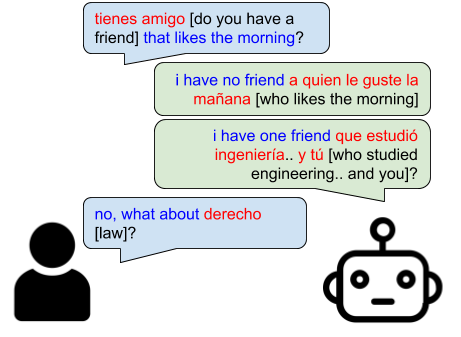
\includegraphics[width=0.48\textwidth]{img/ex_chat_1101}
	\centering
  	\caption{We build a bilingual goal-oriented system that can converse in Spanish--English CM with human users. In controlled settings, we collect human--computer conversations that enable us to study contextualized code-mixing preferences of the participants.}
    \label{fig:human-comp-chat}
\end{figure}

In order to study code-mixing in a controlled setting, we began by modifying an existing goal-oriented dialogue framework from \citet{He2017} to handle different strategies of Spanish--English CM.
We used their scenario of discussing mutual friends given a knowledge base. 
According to this framework, both users of the system (in our case, one human and our rule-based agent) had a private table of friends with certain attributes. 
Only one friend appeared in both tables, and the goal was to select that mutual friend via collaborative discussion over text chat.
The benefit of this symmetric collaborative dialogue is that it is goal-oriented, while remaining flexible in the topics of discussion.
% Sai: In brief / In summary / [sth else], this setting / framework is both flexible in ... as well as task oriented
An example is visualized in \Fref{fig:human-comp-chat}.

To generate text, we added modifications (visualized in green in \Fref{fig:sys-diagram}) to the original monolingual generation (in blue). 
The rule-based agent generated English strings, which were passed to an Automatic Machine Translation (MT) system in order to receive the Spanish translations. 
With parallel English and Spanish utterances, our strategy transformations output a CM utterance.
For the entire duration of a single dialogue, strategy conditions remained constant.

To process text from users, utterances were first passed to the MT whose target language was English.
% \footnote{This is fairly robust in converting Spanish or mixed Spanish and English into mostly English tokens} \yt{I don't like this footnote, it's too subjective. It would be better to sample 50 examples and manually check the accuracy and report the number.} 
The monolingual dialogue system received English strings via the knowledge base that breaks utterances into basic entities, and this informed the next turn from the agent.
% and checks if any items from the knowledge base were mentioned in order to formulate 
% In our version, we update the knowledge bases and system output to be bilingual. 
% We limit our attributes to school majors, hobbies, locations, and preferred time of day. 
Named entities, as well as word pairs that have the same spelling in both English and Spanish, were avoided so that every item could be classified as clearly English or Spanish (e.g. remove `the piano' / `el piano').

% [h] means place fig "here", t=top, b=bottom
\begin{figure}
	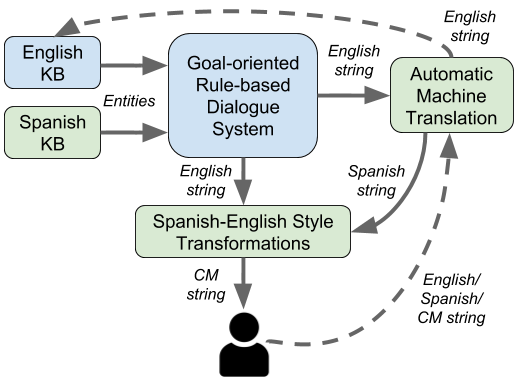
\includegraphics[width=0.48\textwidth]{img/all_system_1031}
	\centering
  	\caption{We add bilingual modules (in green) to the existing monolingual rule-based generation (in blue). The main dialogue system generates CM text via MT and a strategy transformer. It receives user text via translation into English.}
    \label{fig:sys-diagram}
\end{figure}


\section{Code-Mixing Strategies}
\label{sec:strategies}
Based on prior work in CM, we chose to implement our dialogue system to produce text using three specific strategies, namely Content, Structure, and Social. 
Content and Structure originate from \citet{muysken2000bilingual}, and our integration of Social style is a novel approach.
With these conditions integrated in our system, we could analyze the different ways in which users respond to such conditions.

\subsection{Strategy: Content CM}

The first strategy, inspired from \citet{muysken2000bilingual}, is \textit{Insertion}.
This follows the Myers-Scotton framework of a Matrix Language (MatL) and an Embedded Language (EmbL), where the structure and grammar of the MatL is maintained while inserting the EmbL (often single words or phrases) in certain spots \citep{myers1993common}. 
According to \citet{Joshi1982}, closed class items such as determiners, quantifiers, etc. would remain in the MatL.
% prepositions, possessives, auxiliaries, tense, helping verbs,
This has been shown to be more commonly used when the speakers are not equally proficient in both languages \citep{Deuchar2007}. 

We defined our first strategy, Content CM, along the same vein as Insertion.
We retained the grammar of English while inserting Spanish nouns, or use Spanish grammar while inserting English nouns (Example 1). 
We will refer to the former version as \textit{EN gram} and the latter as \textit{SP gram}.

\subsection{Strategy: Structure CM}

Muysken also coined \textit{Alternation}, which is when CM adheres to constituent boundaries \citep{sankoff1981formal} and can separate topics or sentences \citep{Ardila2005}. 
This has been shown to be more prevalent among fluent or highly proficient bilinguals as a form of more stable bilingualism \citep{Deuchar2007}. 
We also incorporated the functional head constraint from \citet{Belazi1994}, where switch points can occur between the lexical head and complement (Example 2a).
% in types of Structure CM generation

We used these priors to inform our second strategy, Structure CM, where the agent either begins in English for a phrase and then switches to Spanish, or begins in Spanish and then switches to English (Example 2b).
We will refer to the first as \textit{EN\textrightarrow SP} and the second as \textit{SP\textrightarrow EN}.

\subsection{Strategy: Social CM}

We defined our third strategy, Social CM, to have added discourse markers on top of either Content or Structure strategies.
% Lastly, since CM can occur more in casual dialogue and between people who have good rapport, 
Discourse markers are actively used by speakers in improving the flow of dialogue, and they remain relatively independent of syntax or semantics \citep{schiffrin1988discourse}.
Within CM speech, these markers can be adopted as an easy form of lexical borrowing by bilinguals of varying proficiency.
In particular, Spanish markers within English speech can be used to signify a less formal tone or to reveal Latino social identity \citep{Torres2011}.
Example 3 shows the use of \textit{you know} as the English discourse marker in a CM utterance.

Using this knowledge, we checked the coverage of a set of markers\footnote{This set of common English and Spanish markers are curated from online sources and native informants.} in the Miami Bangor corpus, keeping those that occur with a frequency greater than 1\% of the tokens within CM utterances. 
We added these markers in either utterance-initial or utterance-final position.
In total we had 6 Spanish markers, 4 English markers, and 4 bilingual markers.\footnote{Additionally, we converted all numbers from numerals to text, lowercase all utterances, and sometimes add extra punctuation like ``!'' and ``...''.}
% From the existing 4 strategies (2 from each of Content and Structure), we expand to a total of 8 CM conditions.


\begin{itemizesquish}
\item Example 1 -- Content (\textit{SP gram}): ``\textit{Me confirm\'o Juan que fue muy obvio, y no solamente en la} [Juan confirmed to me that it was very obvious, and not only in the] produce section, \textit{tambi\'en en el} [also in the] check-out line.'' \cite{Solorio2008}
\item Example 2a -- Structure: ``\textit{la mujer} [the woman] proud of her position'' \cite{Belazi1994}
\item Example 2b -- Structure (\textit{SP\textrightarrow EN}): ``\textit{Yo no estoy de acuerdo con eso.} [I am not sure about this.] But, anyhow, I think I will try again to get it.'' \cite{Ardila2005}
\item Example 3 -- Social: ``\textit{Yo estaba aburrecido, muri\'endome,} [I was bored, dying,] you know?'' \cite{sankoff1981formal}
\end{itemizesquish}

\subsection{Presence in other corpora}
\label{ssec:miami-twitter}

To verify the coverage of these types of CM, we analyzed their prevalence in two separate Spanish--English corpora: the Miami Bangor corpus of transcribed spontaneous speech \citep{deuchar2014building}, and the Twitter corpus from the 2016 Language ID shared task \citep{Molina2016}. 
% Each corpus has been tagged with the language ID. \ea{continue}. 
These distributions are given in Table \ref{tab:strategy-mb-twitter}, and the heuristics to automatically classify the strategies are discussed in Section \ref{ssec:eval_method}.\footnote{The 3 strategies may have overlapping distribution. 
The way we calculated and reported values across other corpora was by checking for Structure first, then Content. 
Social was not directly measured, and we only report 1 strategy per utterance.} 
We see that the most common strategy is Content CM, specifically \textit{SP gram}, which follows findings from a Spanish--English corpus of blogs from \citet{Montes-Alcala2007}.

\begin{table}
\begin{center}
\begin{tabular}{l|cc}
\hline \bf Strategy & \bf Miami Bangor & \bf Twitter \\ \hline
\textit{SP gram} & 29.98\% & 45.53\% \\
\textit{EN gram} & 16.13\% & 11.33\% \\
\textit{SP\textrightarrow EN} & 16.54\% & 12.91\% \\
\textit{EN\textrightarrow SP} & 12.26\% & 13.73\% \\
neither & 25.10\% & 19.25\% \\
\hline
\end{tabular}
\end{center}
\caption{\label{tab:strategy-mb-twitter} We verified that two of our CM strategies, Content and Structure, had a presence in two corpora.
Values were calculated on the assumption that all analyzed utterances were tagged with English and Spanish.}
\end{table}


\subsection{Research Questions}
\label{ssec:research-questions}
%\ea{Changed from `Hypotheses'... convert to full sentences, maybe numbered?}
Armed with bilingual collaborative settings that operationalize 
linguistically-motivated CM strategies, 
%Given these strategies, 
we will analyze (1) how users' \emph{choice of CM} varies, 
(2) how much they \emph{entrain} to the agent, 
and (3) both the \emph{extrinsic task success} and the \emph{perceived success} of the dialogues.
To analyze the users' choice of CM and their entrainment to our 
dialogue agent, we explore the following research questions:  
\begin{itemizesquish}
\item Will certain strategies elicit more CM than others? Will they affect task or dialogue success?
\item Do the user CM strategies follow the same distribution as in existing datasets? Can system conditions change the distribution by entraining users?
\item Will the added Social strategy result in more or less entrainment of user CM style? Will it result in higher task or dialogue success?
\item How do language proficiency, gender, and age affect user CM strategies?
\end{itemizesquish}


\section{Experimental Settings}
\label{sec:experiment}
In order to examine effects of different CM strategies with human bilingual speakers, we chose to modify an existing dialogue system (\Sref{sec:dialogue-system}) and deploy it to chat with crowdworkers.
%The methodology is described below.

\subsection{Data Collection}

We released this task on two crowdsourcing platforms: Amazon Mechanical Turk\footnote{https://www.mturk.com/} and Figure Eight\footnote{https://www.figure-eight.com/, originally CrowdFlower.}. 
In order to target Spanish--English bilinguals, we limited workers to be in the US,\footnote{Other countries were not included in order to limit the variance of social and cultural factors for Spanish--English CM.} and then included several ungraded Spanish proficiency test questions. 
Additionally, the introduction and instructions to the task were purely written in Spanish to prime the user in both languages, given that English is usually the default language for tasks released in the US. 
An example of the interface shown to the user is given in Figure \ref{fig:interface}. 
In addition to the 8 CM conditions, we had 2 more monolingual conditions (Spanish and English), as well as a Random CM condition where a switch point could occur with 50\% chance at every smallest word unit.
For each chat, there were always 10 friends, 3 attributes. Additionally, there was a timer for 8 minutes within which the user had to complete the task.

\begin{figure}
    \centering
	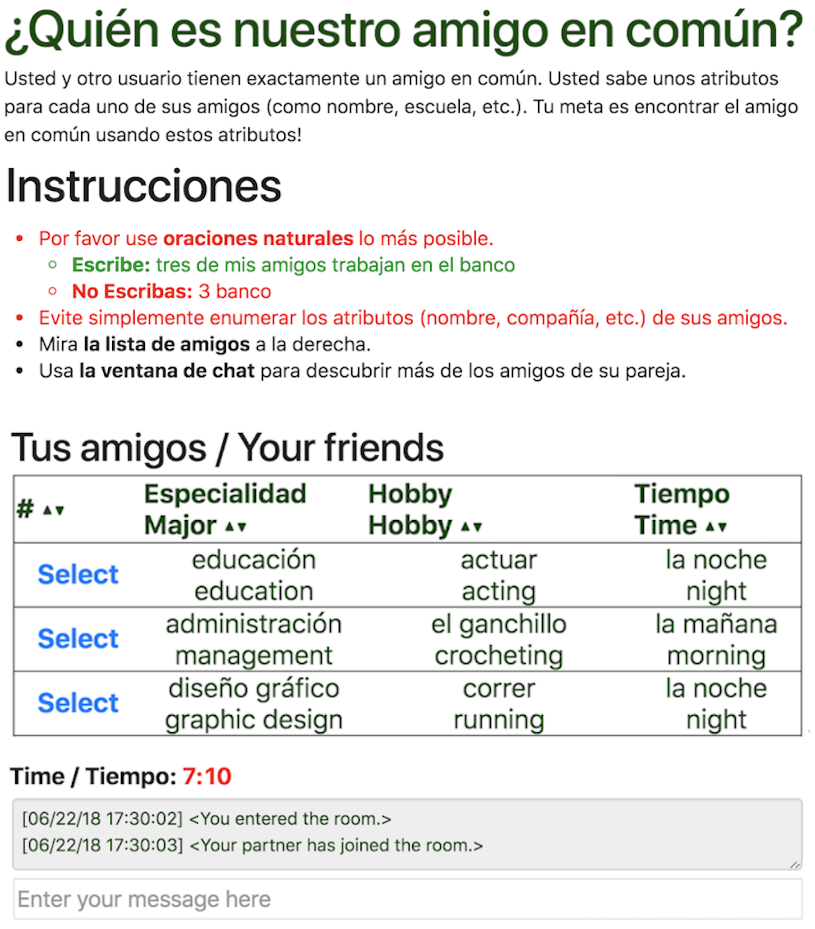
\includegraphics[width=0.48\textwidth]{img/interface_1101_2}
  	\caption{Crowdsourced users would see an interface similar to this when chatting with our dialogue system via text. Unique features include the bilingual table of friend attributes.}
    \label{fig:interface}
\end{figure}

\subsection{Evaluation Methodology}
\label{ssec:eval_method}
Once all data was collected, we used a few heuristics in order to analyze the amount of CM and the type of CM in a given message.

\paragraph{Language Identification}
Tagging utterances with language identification on the token-level is crucial for measuring amounts and strategies of CM.
In order to classify tokens as English, Spanish, or neither/ambiguous, we created separate dictionaries for Spanish and English.
Each dictionary contained vocabulary from our domain knowledge bases as well as from the top 1000 most frequent words from each language.
If tokens existed in the dictionary, they would be tagged as that language, and tiebreakers of entries that appeared in both languages defaulted to Spanish. 
After this automatic check, we combed through the data and manually fixed language ID tags.
% \footnote{The tokens that needed manual fixing were typically spelling typos, homographs that appear in both languages (e.g. \textit{a} and \textit{me}), and inflections of common verbs (e.g. \textit{estudie/estudiado}).}

\paragraph{Strategy Classification}
We introduce a novel method to classify CM utterances into one of four strategies:  \textit{EN\textrightarrow SP}, \textit{SP\textrightarrow EN}, \textit{EN gram}, and \textit{SP gram}.
% Social strategy is not directly measured.
% \footnote{Note this is the same metric used to c alculate strategies in the Miami Bangor and Twitter corpora.}

An utterance is a Structure switch from Lang\textsubscript{A} to Lang\textsubscript{B} if there is at least one Lang\textsubscript{A} function word followed by at least one Lang\textsubscript{B} function word.
Since function words are closed class items and indicators of the MatL \citep{Joshi1982}, we are ensured that the MatL is switching after a full phrase and thus counts as Structure CM.

If the utterance is not classified as Structure, it is next tested for Content.
We define Content CM to occur under two conditions: (1) the MatL has more function words than the EmbL, and (2) the EmbL has at least one content word.\footnote{Content is defined as one of [`NOUN', `ADJ', `VERB', `PROPN'] from Myers-Scotton's framework. We generated POS tags from English and Spanish POS taggers provided by Spacy, available at https://spacy.io/.}
This metric ensures maintaining the grammar of the MatL with insertions of the EmbL.
% \ea{Do I need to show the ``goodness'' of this classification technique?}
% \yt{it would be good, but not sure how to evaluate it quantitatively. maybe at least some justification or examples?}

\section{Results and Analysis}
\label{sec:results}

After running experiments and processing the text, we present exciting main findings of our new CM corpus.
We then examine the subtleties of how users code-mixed under different conditions.
Our questions from \Sref{ssec:research-questions} guide us in our analyses of strategy conditions, dialogue success, levels of entrainment, and demographic factors.

\subsection{Collected Dialogues}
We report general statistics of our collected dialogues in Table \ref{tab:overview-stats}.

\begin{table}[]
\centering
\begin{tabular}{ll}  % l
\hline
\# Dialogues                     & 587    \\
\% Extrinsic Task Success        & 64\%   \\
Avg \# user utterances           & 7.9   \\
Avg \# tokens / utterance        & 6.2   \\
% following # is for entire turk task, not simply time w/ chatbot
% avg time per task (min)          & 10.1    \\
EN vocab size                    & 571    \\
SP vocab size                    &  846    \\
\% EN utterances                 & 16\%   \\
\% SP utterances                 & 44\%   \\
\% CM utterances                 & 39\%   \\
\% dialogues w/ CM               & 70\% \\
\hline
\end{tabular}
\caption{Our bilingual corpus of crowdsourced conversations has a strong presence of CM.}
\label{tab:overview-stats}
\end{table}
% Old caption: General statistics of our dataset. Success here is the extrinsic task success of finding the mutual friend or not.

A total of 737 dialogues were collected, but 587 remain for analysis. We removed 112 chats because they contained no text from users\footnote{Not typing back to the dialogue system was allowed, and users could click on different friends until they achieve the extrinsic goal.} and another 38 because the users did not take the survey.

From the pool of 587 valid chats, there were 296 unique workers because some did more than one task. 
The self-reported survey revealed that the mean age for the workers was 31, 60\% of them were male, and the most frequently reported countries of origin were USA, Venezuela, and Mexico.

Examples of conversations gathered with crowdsourced bilinguals are given in Table \ref{tab:example-dialogues}.
% of our dialogue system
An interesting observation is that the user chose to emulate the strategy instead of echoing that lexical item in the \textit{SP\textrightarrow EN} Structure condition.
Even when the agent used the Spanish word \textit{contabilidad}, the user said the equivalent meaning in English, which is \textit{accounting}.
In the same way, when the \textit{SP\textrightarrow EN} agent discussed \textit{dancing}, the user replied with the Spanish equivalent, \textit{bailar}, thus prioritizing strategy over lexicon.

% EXAMPLE CONVERSATIONS
\begin{table*}[t]
\centering
\begin{tabularx}{\linewidth}{sb|sb}
% \toprule
\hline
\multicolumn{2}{c}{\bf\textit{EN\textrightarrow SP}} & \multicolumn{2}{c}{\bf\textit{SP gram}} \\
\hline
A: & I have 2 friends \textit{que estudiaron la contabilidad} [that studied accounting] & A: & \textit{?`Tiene} [Do you have] friends \textit{que trabajen en el} [who work at the] theater \textit{o un} [or a] friend
\\

H: & \textit{yo tambien} [me too]. one that studies accounting \textit{trabaja en el concesionario de coches y el} & & \textit{que trabaje en la} [that works at the] jewelry store ?
\\

& \textit{otro en la oficina} [works at the car dealership and the other in the office] & H: & \textit{si. la del} [yes. the one from] jewelry store \textit{le gusta dormir} [likes to sleep]
\\

A: & Do you have any friend who likes dancing \textit{o amigos a los que les guste hornear} [or friends who like to bake]? & A: & \textit{tengo} [I have] 1 friend \textit{que le gusta} [who likes] acting, 1 friend \textit{que trabaja en el} [who works at the] zoo
\\


H: & \textit{nadie le gusta bailar} [no one likes to dance]. one likes baking--\textit{el/ella estudia fisica} [he/she studies physics] & H: & \textit{la del teatro le gusta} [the one from the theater likes] photography
 \\


% \bottomrule
\hline

\multicolumn{2}{c}{\textbf{\textit{SP\textrightarrow EN +SOC}}} & \multicolumn{2}{c}{\textbf{\textit{EN gram +SOC}}} \\
% \midrule
\hline
A: & \textit{tengo un amigo} [I have a friend] who studied english.. \textit{y t\'u} [and you]? & A: & do you have any \textit{amigos} [friends] who studied \textit{derecho} [law] ?
\\
H: & \textit{no tengo... solo tengo un amigo que estudio} [I & H: & no i don't
\\

 & don't have... I only have a friend that studied] linguistics & H: & \textit{tienes un amigo a quien le gusta cocinar} [do you have a friend who likes to cook]?
\\

A: & hey \textit{tengo dos amigos} [I have two friends] who like sewing & A: & nah i have no \textit{amigo} [friend] who likes \textit{cocinar} [to cook]..
\\
H: & \textit{yo tengo un amigo que le gusta} [I hve a friend that likes] sewing! & &
\\
%   \bottomrule
\hline
\end{tabularx}
\caption{\label{tab:example-dialogues} These examples from our corpus of human (H) interactions with CM Agents (A) show a diversity of CM strategies.}
\end{table*}

% GENERAL TABLE by strategy
\begin{table}[]
\centering
\begin{tabular}{p{1.5cm}p{0.7cm}p{0.7cm}p{0.7cm}p{0.7cm}}
% \hline
\textit{Agent} & \rot{\# Dialogues} & \rot{\% Success} & \rot{Avg Utts} & \rot{Avg Tokens} \\ \hline
Average         & 53.4        & 64       & 7.9     & 6.2       \\
Std Dev          & (7.8)         & (11)       & (0.9)     & (0.4)       \\ \hline
\textit{SP gram}         & \textbf{70}           & \textbf{47}       & 8.4     & 6.3       \\  
\textit{+SOC}    & \textbf{44}           & \textbf{77}       & 7.4     & \textbf{5.7}       \\
\textit{EN gram}         & 58           & 62       & 7.2     & \textbf{6.9}       \\  
\textit{+ SOC}   & \textbf{44}           & 64       & 8.6     & 6.0       \\ \hline
\textit{SP\textrightarrow EN}           & 54           & 74       & 7.5     & 6.4        \\  
\textit{+SOC}      & 56           & \textbf{45}       & \textbf{9.7}     & 6.1       \\
\textit{EN\textrightarrow SP}           & 55           & \textbf{76}       & 7.9     & 6.3       \\  
\textit{+SOC}      & 47           & 64       & 7.7     & 6.1       \\ \hline
\textit{Mono SP}         & 46           & 72       & 7.2      & 6.1       \\
\textit{Mono EN}         & 54           & 69       & \textbf{6.4}     & 6.5       \\ \hline
\textit{Random}          & 59           & 64       & 8.2     & \textbf{5.3}       \\ \hline
\end{tabular}
\caption{Grouped by agent strategy, these general statistics show dialogue quantity, length, and success of users. Values further than 1 standard deviation away from the mean are in \textbf{bold}.}
\label{tab:general_tbl}
\end{table}

Based on numbers in the general information found in \tref{tab:general_tbl}, we recommend that if future CM dialogue systems desire to be efficient in number of turns, the \textit{EN gram} strategy is useful, but if they want to chat for longer, \textit{EN gram +SOC} or \textit{SP\textrightarrow EN +SOC} could yield more turns.


% \section{Analysis}
% \label{sec:analysis}


\subsection{Types of User Code-Mixing}
% \ea{use more excited language, frame how cool this is!}
Our first encouraging finding is that a high majority of dialogues contain CM from the user (Table \ref{tab:overview-stats}), although the users were not explicitly instructed to code-mix. This implies that code-mixing is a preferable communication style and that conversational agents could benefit from supporting multilinguality.  
The questions now are how much CM did the users do, how did they do it, and how much did the agent strategy conditions factor into response style?


% CM TABLE by strategy
\begin{table}[]
\centering
\begin{tabular}{p{1.5cm}p{0.7cm}p{0.7cm}p{0.7cm}p{0.7cm}}
\textit{Agent} & \rot{\% Dial. w/ CM} & \rot{\% Utts = CM} & \rot{M-idx} & \rot{I-idx} \\ \hline
Average         & 70        & 39       & 0.74     & 0.23       \\
Std Dev          & (8)         & (8)       & (0.20)     & (0.04)       \\ \hline
\textit{SP gram} & 74           & 42       & \textbf{0.51}     & 0.23       \\
\textit{+SOC}    & \textbf{80}           & 44       & 0.57     & 0.26       \\
\textit{EN gram} & 74          & \textbf{52}      & 0.93     & 0.26       \\
\textit{+ SOC}   & 75           & 37       & \textbf{0.99}     & 0.26       \\ \hline
\textit{SP\textrightarrow EN}  & 76          & 39       & 0.88     & 0.24        \\
\textit{+SOC}    & 75         & 40       & 0.71     & 0.26      \\
\textit{EN\textrightarrow SP}  & 71          & 40      & 0.91     & 0.23       \\
\textit{+SOC}    & 72          & 37       & 0.70    & 0.23       \\ \hline
\textit{Mono SP} & \textbf{57}          & \textbf{26}       & \textbf{0.37}      & \textbf{0.16}       \\
\textit{Mono EN} & \textbf{54}          & \textbf{25}       & 0.74     & \textbf{0.16}       \\ \hline
\textit{Random}           & 66          & 39       & 0.86     & 0.22       \\ \hline
\end{tabular}
\caption{These statistics quantify users' amount of CM under different agent strategies. Values further than 1 standard deviation away from the mean are in \textbf{bold}.}
\label{tab:cm_strategy}
\end{table}


We first analyze the amount or presence of CM from the users. 
\citet{guzman2017metrics} defined several metrics based on quantifying token counts and span lengths of continuous monolingual tokens.
The Multilingual-index (M-idx) reflects how balanced the tokens are in each language, where 0 is fully monolingual and 1 is an equal number of tokens per language. 
The Integration-index (I-idx) is the probability of switching languages between any two tokens, where 0 is fully monolingual and 1 is a perfectly interleaved corpus, with a switch at every word.\footnote{To calculate I-idx in a given dialogue, all utterances by one party (either user of our dialogue agent) were collapsed in order, so switch-points can occur across utterance boundaries.}
Higher values of both indices imply a higher quantity of mixing. 

% \yt{rephrased because "parallel corpus" term is not clear in this context. parallel corpus is when every sentence appears in both languages, sentence-aligned.}

From \tref{tab:cm_strategy}, we see that \textit{EN gram +SOC} and Structure conditions resulted in higher M-indices than average. 
Most notably, the \textit{SP gram} condition resulted in the lowest M-idx and I-idx from users.
This was due to receiving more monolingual Spanish text from users than in any other condition, a potential result of having the crowdworkers primed to be in Spanish mode.
Conversely, the \textit{EN gram} conditions maintained markedly high CM indices from users.
Under the logic that users were primed more in Spanish, \textit{EN gram}, the agent with the highest number of English tokens could have encouraged users to balance their Spanish tokens with more English.
We advise future CM systems to be aware of their target audience's backgrounds and primed default languages.


% \ea{Maybe TODO: discuss \%s of presence of CM/Spa/Eng utterances
% Compare distribution with Miami/Twitter}

% \ea{Maybe TODO: within group effects of conditions, vs random baseline.}

\subsubsection{Entrainment}
We now analyze if users were entrained to the agent---whether they copied the amount of CM or the CM strategy of the agent.
\begin{figure}[!h]
	\centering
	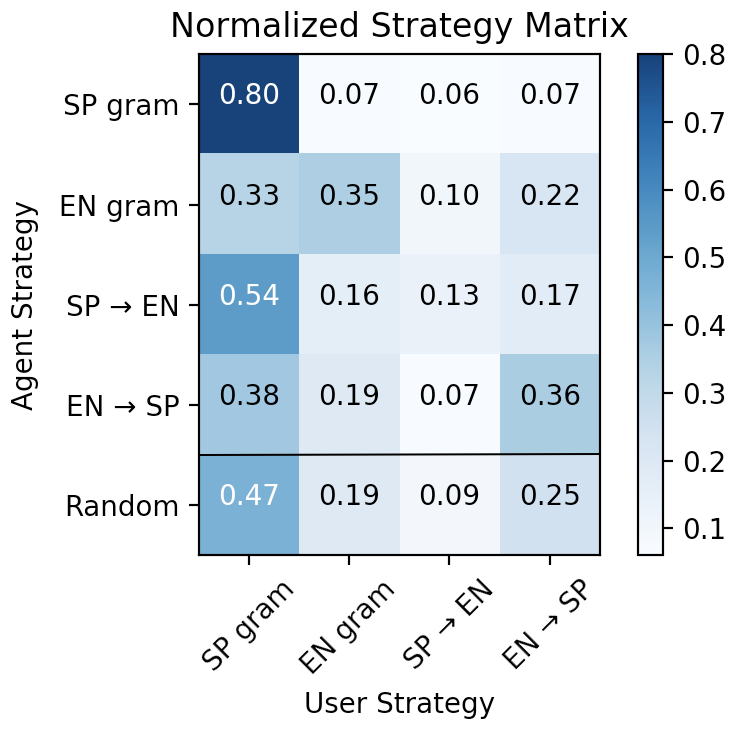
\includegraphics[width=0.48\textwidth]{img/1031_entrain}
  	\caption{We find entrainment in our data. Given each agent strategy condition (per row), we display the normalized distribution of which strategies the users used (only accounting for utterances that are code-mixed). Darker colors along the major diagonal indicates complete entrainment, and the random agent strategy at the bottom is shown for comparison.}
    \label{fig:entrain_matrix}
\end{figure}

\paragraph{Quantity of CM}
An intuitive assumption is that Structure-based CM has a lower I-idx since switches are likely to be more periodic and less frequent.
Yet, while the Structure strategies from the agent produced utterances with lower I-indices, the same pattern was not found in users' responses. 
Users had a stable I-idx across all CM conditions and thus did not entrain to the agent's I-idx. 
As for M-idx, the Structure conditions produced utterances that were nearly at 1.0, which is higher than the Content conditions. 
However, we did not see this trend in the users---M-idx was low for \textit{SP gram}, medium in Structure conditions, and highest for \textit{EN gram}.
Presumably, since \textit{SP gram} was the strongest strategy to be repeated back, the quantity of English tokens would be much less (thus, a lower M-idx). 

\paragraph{CM Strategy}
We see the presence of entrainment between agent strategy (condition) and user strategy.
% from the metrics we defined in Section \ref{ssec:eval_method} to classify a CM utterances into strategies, 
In the matrix in \Fref{fig:entrain_matrix}, perfect entrainment (where all the users' CM utterances use the same fixed agent strategy) would be shown with a normalized value of 1.0 along the diagonal. 
We compared values across CM conditions (without examining \textit{+SOC} for now) to the random baseline, which ideally revealed the natural unconditioned distribution of user strategy.\footnote{Reassuringly, the percentages in this random condition are similar to the distribution of the Miami Bangor and Twitter corpora from \tref{tab:strategy-mb-twitter}.}
Because the values on the diagonal were greater than in the random condition, we infer that the agent consistently influenced the user's code-mixing.

Upon closer inspection, \textit{SP\textrightarrow EN} was the least common strategy from users, as well as the weakest strategy to be entrained. 
In that agent condition, more of its user utterances were being classified as \textit{SP gram}, which was at least consistent with the agent's starting MatL.
For the conditions where English was the main (or starting) MatL, \textit{SP gram} occurred less often, while other English-based CM strategies were used more often. 
There was also more sensitivity to the specific English strategy because more utterances were classified as \textit{EN gram} in \textit{EN gram} conditions and \textit{EN\textrightarrow SP} in \textit{EN\textrightarrow SP} conditions.
Overall, \textit{SP gram} was the most popular strategy used---it was most common in the \textit{SP gram} condition, but still kept strong presence in the other conditions.
We recommend \textit{SP gram} to be a good default strategy in future CM agents, as that also follows the prevalent styles in the Miami Bangor and Twitter corpora (\Sref{ssec:miami-twitter}).

\subsection{Dialogue Success}

We define two types of Success in the dialogues:

\begin{enumerate}
\item Extrinsic success (the binary extrinsic goal of finding the mutual friend in the given 8 minutes).
\item Perceived success (self-reported measures on an agreement scale of 1-5, e.g. \textit{``I understood the task perfectly''}, or \textit{``My task partner texts like someone I know''}).
\end{enumerate}

\paragraph{CM Strategy}
From \tref{tab:general_tbl}, both Structure conditions and both monolingual conditions achieved consistently high rates of extrinsic task success.
This could reveal that longer spans of monolingual tokens aided in users comprehending the task, so we recommend CM systems to adhere to Structure strategies if they desire specific goals to be achieved.

\paragraph{Quantity of CM}
Using Pearson's $r$, we then examined if the quantity of CM or the level of entrainment have correlations with both types of success.
All results were considered significant with $r^2 > 0.2$.

While user M-idx and I-idx did not correlate with the binary extrinsic goal, M-idx negatively correlated with number of turns in the dialogue ($p < .001$).
% This means that in quicker chats there was less balance of tokens in both languages.
% Although quicker chats could mean the user succeeded in finding the friend early, there was no significant negative effect of extrinsic goal.
Intuitively, there could have been less chance for mixing when the user spoke across fewer turns.
As for perceived success, when users reported that they understood the task better, M-idx and I-idx were higher ($p < .001$).
It is likely that the task primed users to code-mix.\footnote{The instructions encouraged users to ``use English, Spanish, or a mixture of the two''. The title of the crowdsourced task is also called \textit{``Charlemos en Spanglish!''}, meaning ``Let's chat in Spanglish!''}

\paragraph{Strategy Entrainment}
We quantified an entrainment score within one dialogue to be a ratio of the number of user utterances that copied the given agent strategy, over the total number of CM user utterances. 
Ultimately, we did not find significant correlations between this entrainment score and any type of success metric for the aggregate users.
% This implies that the different agent strategies of CM do not affect the perception of the user, making it more seamless to use different strategies interchangeably. 
Having some opacity in the link between strategy and task success could allow future CM dialogue systems to be diverse in strategy, which gives future work a chance to find more optimal and nuanced ways to incorporate CM into these intelligent agents.

% \ea{Maybe TODO: how does the distribution of our entrainment values compare to those from MIAMI?}

\subsection{Effect of Social CM}
The third dimension of CM, namely the added social/informal strategy, had a number of effects on the other two dimensions.
Across all 4 Content and Structure conditions, it reduced the average number of tokens in the reply from the user (seen in \tref{tab:general_tbl}), which could be a result of users being more casual with the dialogue system.
We now examine this factor with three of the measures discussed previously.

Regarding amount of CM present, when social discourse markers were added, M-idx increased for both Content strategies while sharply decreasing for both Structure strategies.
I-idx slightly increased for all strategies except \textit{EN gram}.
% We hypothesize that 
% \ea{When I look at examples qualitatively, I can't see why this happens... but how to add analysis to these findings?}
Regarding success, the added social and informal strategy did not have a significant effect.

Lastly, for most strategies except for \textit{EN gram}, a more social agent resulted in less entrainment.
% (lower normalized scores along the major diagonal if visualized in a table similar to Figure \ref{fig:entrain_matrix})
We find that the users generally used more \textit{SP gram} in their chat.
The \textit{EN gram} condition was the exception, where \textit{EN gram +SOC} led to users emulating \textit{EN gram} more.

We encourage CM dialogue systems to consider implementing casual styles of speech in CM because simple additions of discourse markers produced patterned changes in token length, amount of CM, and entrainment.
We will, however, show more nuanced effects of Social CM in the following section.



% \ea{TODO: calculate users' amount of socialness (presence of discourse markers)}

\subsection{Effect of User Type}

Beyond analysis of the aggregate data, we found strong effects of the following user attributes.
% \ea{Any confounding factors? platform (MTurk vs Figure 8)?}

\paragraph{Language Proficiency}

% several self-reported metrics, which include a 5-point scale of English and Spanish ability, age one began to learn each of the two languages, and scores from a 3-question quiz\footnote{We passed everyone who took the quiz, and given the location constraint was the US, we did not release an English proficiency quiz.} on Spanish grammar that we created.
Our findings support the hypothesis from \citet{Deuchar2007} in that more proficient bilinguals (balanced in both languages) use Structure strategies more often than asymmetrical bilinguals. 
We examine this by binning the groups into three categories from the self-reported language ability metric\footnote{We measure proficiency as the self-reported scores of users' own English and Spanish ability on a 5-point scale.}: highly proficient in both English and Spanish, dominant English only, and dominant Spanish only.
% both (high ENG and high SPA, 207 users), dominant English (high ENG and low SPA, 77 users), and dominant Spanish (high SPA and low ENG, 29 users)
Compared to the aggregate report of user CM, dominant English speakers use \textit{EN gram} more heavily, while dominant Spanish speakers use \textit{SP gram} more heavily.
Structure CM occurs in those two groups but is more present in the balanced bilingual group.
% Although the quantity of chats for the asymmetrical bilinguals is low, our findings support the original hypothesis.

For the dominant English speakers, a higher M-idx correlated with better agreement on statements such as \textit{``My task partner was very cooperative''} ($p < .05$).
When these users entrained more to the agent's CM strategy, the number of turns in the dialogue also increased ($p < .05$). 
Also, even though extrinsic task success for them was low on the monolingual Spanish condition, all CM conditions (except \textit{SP\textrightarrow EN +SOC}) boosted task success.
Together, these findings show that the dialogue experience overall improved for less-balanced bilinguals when the agent used CM, especially as compared to a monolingual agent of their weaker language.
This supports a line of pedagogy that supports incorporation of CM in second language instruction~\citep[cf.][]{moore2002code}.
% \ea{not enough dialogues, only 2-6 per condition, to make conclusions for dominant Spanish speakers.}

\paragraph{Demographic Factors}
Reported gender\footnote{``Other'' gender constituted 1\% of users and was set aside for this analysis.} yielded strong correlations in user CM strategy.
For females, higher M-idx and I-idx significantly correlated with higher agreement on the statement \textit{``I am very likely to chat like I did in this task when messaging with my bilingual friends''} ($p < .005$).
This finding both reflects that females code-mixed naturally and highlights the potential for future CM dialogue systems.

% , women on average had a slightly higher M-idx (by .06), yet an identical I-idx.
Females responded to social conditions such that they had longer dialogues and more CM, which proved to be an opposite effect for males.
With the social discourse markers, females consistently had higher percentages of CM utterances than males (a difference of 4-11\% for each condition).
Yet, without social strategy, men had equal or higher percentages of CM utterances than women (an exception being \textit{EN gram}). 
This same pattern can be seen in \% dialogues containing CM where women had higher values in social condition while men had the reverse, but the exception for men was that for \textit{SP gram}, women still had more CM dialogues than men (though less strongly than in \textit{SP gram +SOC}.
Again this held for number of utterances per dialogue. 
With added social strategy, women had 1-3 extra utterances while without social strategy, the men had more utterances (again with one exception that in \textit{SP\textrightarrow EN}, women still had more utterances than men, but less strongly than in \textit{SP\textrightarrow EN +SOC}).
% \ea{Do I need to support previous stats with \#s in a table?}

In addition to gender, reported age also affected user styles.
We used a threshold of 35 to split users into younger and older age categories, with the latter group yielding 22\% of all dialogues.
Compared to older users, younger users on average achieved extrinsic success 12\% more often, used more CM, and had longer conversations (more utterances, but slightly less tokens per utterance).

% \paragraph{User Response Style}
% \ea{Would this sub-section be interesting? I haven't calculated these things yet.}
% What happens when user uses certain strategies? When user uses short vs long utterances? 
% More or less turns? 
% More punctuation and capitalizing text (indicating formal style)? 
% Amount of CM and CM strategy?

\subsection{User Feedback}
Users of this study overall had positive impressions of their dialogue experience.
They mostly agreed to the statement \textit{``If technology (like Siri or Alexa) progressed to allow me to use Spanglish, I could see myself using both languages with it''}, and this is an encouraging sign for future systems that want to incorporate Spanish--English CM in their dialogue.
%  (aggregate 4.14/5.0, meaning ``Mostly Agree'')

A common critique we received was similar to this user's experience: ``my partner was all over the place. It was hard to keep up with all their \textit{preguntas} [questions]. I don't think we ever found our \textit{amigo en comun} [mutual friend].''
Given that our agent is rule-based, it could often dominate the conversation and lead users down specific dialogue patterns, but this was an expected trade-off to allow for fine-grained control of system output.
There is room for future work to incorporate bilingual code-mixing into more advanced dialogue systems like the knowledge graph-based system from \citet{He2017}.

Another valuable comment validated several of our goals.
A user who had the \textit{EN gram +SOC} agent said, ``in my experience speaking with other bilingual friends the switching is usually either half of the sentence or alternating sentences... Rarely do I just use one word in the other language unless it's pretty specific to that language... But I found myself doing it along with the robot!''
They acknowledged that they would naturally use a more alternating, Structure strategy of CM, but instead entrained to the agent who used a Content strategy.


\section{Related Work}
\label{sec:related-work}

We provide a brief overview of previous works in the domains of code-mixing and dialogue.

% From fields of NLP and Linguistics,

Attempts have been made to integrate CM into NLP areas such as Part-of-Speech tagging \citep{Solorio2008,soto2018joint}, Language Identification \citep{soto2018joint,Rijhwani2017}, Named Entity Recognition \citep{aguilar2018named}, Language Modeling \citep{chandu2018language}, Automatic Speech Recognition (ASR) \citep{yilmaz2018building}, and Speech Synthesis \citep{Rallabandi2017}.
There also has been a push to generate CM datasets synthetically to improve CM language modeling \citep{pratapa2018language}, or manually crowdsource CM utterances towards CM Question--Answering and dialogue systems \citep{chandu2018code,banerjee2018dataset}.
% Code-mixed corpora are emerging, such as the code-mixed DSTC2 restaurant reservation dataset where crowdworkers manually translated from English into various Indian Englishes---this dataset was built with the intention of developing future goal-oriented dialogue systems \citep{banerjee2018dataset}.
% Our corpus differs in that one partner is an agent while the other is responding to this specific scenario in real-time.

% Another ASR paper from 2017: Amazouz2017, sivasankaran2018phone
% predict switch points from one language into another
% \citet{Fricke2016} also discovered the importance of acoustic cues in determining when users will code-switch.
% Pratapa et al. (2018) used syntactic linguistic theory to generate synthetic code-switched data, which could aid in CM language models ().

Various other research has centered around understanding when and why people code-switch.
Linguistically-driven methods have found that cognates and acoustic cues allow for more fluid switching between the languages \citep{kootstra2012priming,Fricke2016}.

When pertaining to a dialogue setting, CM has been found to fulfill different goals of speakers \citep{begum2016functions}. \citet{Solorio2008} discussed how sociopragmatic factors, such as the topic being discussed and the rapport between the speakers, could influence the style of CM.
In support of this, \citet{Yoder2017} showed that the use of code-mixed English marked positive social influence in a study of Arabic Wikipedia editor talk pages.
Additionally, choosing to use one language over another can be a pragmatic way to mark sentiment, as \citet{rudra2016understanding} found in Hindi--English Twitter data.
These findings support our aim of understanding CM in nuanced contexts of dialogue.
% and found that Hindi was more popularly used for expressing negative sentiment.

Entrainment in bilingual human--human dialogues has been recorded since \citet{giles1973towards} where French--English speakers would choose their language according to their audience.
More recently in entrainment of CM, \citet{soto2018role} showed a convergence in the quantity of CM between speakers over the course of long conversations in the Miami Bangor data.
\citet{fricke2016primed} also found that the presence of CM can affect the utterance following it.
Our work is the first to identify entrainment of diverse CM strategies.


\section{Conclusion}
\label{sec:conclusion}

% sentences taken from intro. MODIFY:
% In this study, we controllably analyze the different strategies in which people may code-mix in dialogues, in order to pragmatically and linguistically learn what makes for successful CM interactions between humans and computers. 
% A successful human--computer dialogue can be determined in ways such as achievement of an explicit goal, or naturalness of a conversation that indicates better rapport.
% We incorporate linguistically-motivated strategies of CM into a rule-based, goal-oriented dialogue system, and analyze the amount of CM, strategy type, and amount of entrainment that a bilingual user has with respect to the agent strategy conditions.
% With these measures, we present analyses of each strategy's effect on the amount of elicited CM and amount of entrainment with respect to dialogue success.
Through our novel Spanish--English dialogue framework, we succeeded in generating CM utterances to which bilingual users also responded in various forms of CM.
Among other exploratory findings, users generally adapted to the strategies used by the agent, but differed in strategy use depending on their bilingual language proficiency.
Adding discourse markers to make the agent more ``social'' affected the patterns of code-mixing, especially among female participants. 
Finally, extrinsic goal success and perceived dialogue success were not hugely affected by CM strategy, but some effects were found from reported age of users.
% Users favor the \textit{SP gram} strategy, but are adaptable to other strategies when fixed as the system condition.

With this data, follow-up analysis can be done on the types of switch points, investigating for example the simplicity or frequency of the word that is switched or the nature of being a cognate \citep{soto2018role}, or even the cognitive accessibility of switch points words from users' mental lexicon.

We acknowledge that our CM corpus reflects a specific population of users that may not reflect all Spanish--English speakers across the world.
Future work can consider other Spanish--English speakers, as well as other language pairs such as Hindi--English.
It is important to learn how these variations may be linguistically or functionally comparative to our findings.

% , since systems accommodating to a user's style has been shown to provide better user experience and task completion \ea{CITE}.

% Topics of dialogue should also expand beyond the task of discussing hypothetical friends with a limited number of attributes.

The implications of our current work, which revealed which CM strategies were more entrainable than others, could help CM agents to better parse and predict user utterances with a more informed language model.\footnote{This approach is similar to a method where ASR systems that lexically entrain users can lower ASR error rates \citep{levitan2013entrainment}.}
Immediate future work should incorporate different CM strategies dynamically within a single conversation.
Additionally, we could also move towards implementing a CM system that entrains to the user.
From here, we can usher in an era of bilingual dialogue systems that brings human--computer interactions to a more personalized space.
% Other applications include educational purposes.
% Labutov \& Lipson (2014)
% Renduchintala+ (2016)
% ``Macaronic'' interfaces for L2 learning


% \section{Appendices} 
% Anything to move here?


\iftaclfinal

\section{Acknowledgments}
Thank God for funding. Include some nice words to nice people.
\else
\fi

\bibliography{tacl}
\bibliographystyle{acl_natbib}

\end{document}